% Created with jtex v.1.0.20
\documentclass{article}
\usepackage{arxiv}

\usepackage[utf8]{inputenc} % allow utf-8 input
\usepackage[T1]{fontenc}    % use 8-bit T1 fonts
\usepackage{hyperref}       % hyperlinks
\usepackage{url}            % simple URL typesetting
\usepackage{datetime}       % show dates in the title block
\usepackage{booktabs}       % professional-quality tables
\usepackage{amsfonts}       % blackboard math symbols
\usepackage{nicefrac}       % compact symbols for 1/2, etc.
\usepackage{microtype}      % microtypography
\usepackage{graphicx}
\usepackage{natbib}
\usepackage{doi}
\usepackage{xcolor}

%%%%%%%%%%%%%%%%%%%%%%%%%%%%%%%%%%%%%%%%%%%%%%%%%%
%%%%%%%%%%%%%%%%%%%%  imports  %%%%%%%%%%%%%%%%%%%
\usepackage{amsmath}
%%%%%%%%%%%%%%%%%  math commands  %%%%%%%%%%%%%%%%
\newcommand{\CRRA}{\rho}
\newcommand{\uFunc}{\mathrm{u}}
\newcommand{\cLvl}{\mathbf{c}}
\newcommand{\mLvl}{\mathbf{m}}
\newcommand{\yLvl}{\mathbf{y}}
\newcommand{\aLvl}{\mathbf{a}}
\newcommand{\Rport}{\mathcal{R}}
\newcommand{\bLvl}{\mathbf{b}}
\newcommand{\pLvl}{\mathbf{p}}
\newcommand{\DiscFac}{\beta}
\newcommand{\cFunc}{\mathrm{c}}
\newcommand{\vFunc}{\mathrm{v}}
\newcommand{\Alive}{\mathcal{L}}
\newcommand{\Ex}{\mathbb{E}}
\newcommand{\permGroFac}{\Gamma}
\newcommand{\permShk}{\psi}
\newcommand{\tranShk}{\theta}
\newcommand{\pZero}{\wp}
\newcommand{\tranShkEmp}{\xi}
\newcommand{\cNrm}{c}
\newcommand{\RNrm}{\mathcal{R}}
\newcommand{\aNrm}{a}
\newcommand{\mNrm}{m}
\newcommand{\Rfree}{\mathsf{R}}
\newcommand{\rfree}{\mathsf{r}}
\newcommand{\eprem}{\varphi}
\newcommand{\Risky}{\mathbf{R}}
\newcommand{\risky}{\mathbf{r}}
\newcommand{\bqstNrm}{e}
\newcommand{\lqdt}{\ell}
\newcommand{\h}{h}
%%%%%%%%%%%%%%%%%%%%%%%%%%%%%%%%%%%%%%%%%%%%%%%%%%


\hypersetup{colorlinks = true,
linkcolor = purple,
urlcolor  = blue,
citecolor = cyan,
anchorcolor = black}

\title{Life Cycle Modeling is (Almost) \\ Ready for Prime Time}

\newdate{articleDate}{21}{11}{2024}
\date{\displaydate{articleDate}}

\makeatletter
\let\@fnsymbol\@arabic
\makeatother

\author{Christopher Carroll\footnotemark[1]\\
Johns Hopkins University\\Econ-ARK\\\AND
Alan Lujan\\
Johns Hopkins University AAP\\Econ-ARK\\}

% Uncomment to override  the `A preprint' in the header
\renewcommand{\headeright}{}
\renewcommand{\undertitle}{}
\renewcommand{\shorttitle}{}

%% Add PDF metadata to help others organize their library
%% Once the PDF is generated, you can check the metadata with
%% $ pdfinfo template.pdf
\hypersetup{
pdftitle={\@title},
pdfsubject={},
pdfauthor={\@author},
pdfkeywords={},
addtopdfcreator={Written in Curvenote}
}

\begin{document}
\maketitle
\footnotetext[1]{Correspondence to: ccarroll@llorracc.org}

\begin{abstract}
The ``life cycle model'' of optimal saving for retirement is familiar to anyone who has taken an introductory economics class.
When hiring a financial advisor, such people probably think the advisor's job is just to tailor optimal life-cycle-model choices to their particular circumstances.
But academics and advisors know that the advice about both saving and portfolio choice provided by standard academic life-cycle models is deeply problematic -- for example, most such models imply that retirees should plan to run their wealth down to zero or some small amount and then (optimally!) live pension-check to pension-check (at least approximately).
This paper makes the case that recent developments in the economics literature have finally given us the tools and insights required to construct rigorous life cycle models whose advice is sensible.
We provide one example of a simple model that can solve a number of problems by putting wealth in the utility function.
\end{abstract}

\keywords{}

\section{Introduction}

Franco Modigliani and Richard Brumberg (1954)\footnote{\cite{2005}} were the first to propose trying to understand consumer financial choices as optimal responses to the paths of income and of spending needs over the lifetime.
An enormous academic literature has followed their pioneering work (see the \href{/lit-review}{literature appendix} for an expansive summary),
but it has proven difficult to build rational optimizing models that give sensible advice about both life-cycle saving choices and about investment decisions.
That is, the models yield implausible answers to questions about how much wealth should be retained later in life, and how much of one's retirement savings should be invested in the stock market.
Indeed, the subtitle of a recent paper by \cite{Daga_2023} captures the current state of affairs nicely: ``Why Practitioners Have Not Adopted the Lifecyle Model -- Yet''; see also \cite{DeNardi2016d}.

In this paper, we argue that the elements are already available to construct a model that ``practitioners can adopt.''
All that is needed is to combine the relevant academic contributions with some wisdom from practitioners' own experience of advising clients.
Our paper's central contribution is to provide a small \href{https://github.com/econ-ark/life-cycle-prime-time}{open-source computational model} that incorporates some of the features that make it possible to build rigorous optimizing life cycle models whose advice is not obviously wrong.

We begin with a (very) brief literature synopsis, then present a set of models that illustrate the difficulty of matching empirical facts with the life-cycle approach.
We end with our proposed solution, which involves a small twist to the old idea (\cite{carrollWhyDoTheRich}) of incorporating wealth directly in the utility function.

\subsection{Recent Developments in the Literature}

\subsubsection{Computation/Uncertainty/Complexity}

Consumers face many uncertainties: about their own income, stock returns, interest rates, health expenditures, mortality, and much more.
Further complications arise because of liquidity constraints and other financial frictions.

The incorporation of realistic descriptions of these complexities makes computation of the mathematically optimal solution to the consumer's problem is astonishingly difficult.
It is more difficult than, say, the calculation of optimal trajectories for spacecraft, and perhaps comparable to the complexity of figuring out how to drive a car roughly as well as a human (another problem where adequate computational solutions have only recently become available).
The remarkable advance of computational power has now finally made it possible to compute a credible answer to the question ``what saving and portfolio choices are truly mathematically optimal?'' in a context in which the key complexities are properly represented.

\subsubsection{Survey Data on Expectations and Preferences}

Another academic development has been a new openness to the idea that people's beliefs and preferences can be probed by \textit{asking them} about their beliefs and preferences.

In the context of motivations for saving, this leads us to take seriously the answers to a survey question about their `most important' reason for saving that respondents to the Federal Reserve's \href{https://www.federalreserve.gov/econres/scfindex.htm}{Survey of Consumer Finances (SCF)} have been asked for many years.
Among retirees, one answer dominates the rest: ``Liquidity / The Future.''  (See the~discussion~below for details).

A natural interpretation of the importance consumers put on ``liquidity'' is that precautionary saving motives matter for many households, highlighting the need for the aforementioned computational advancements.

The traditional approach to constructing such models has been for economists to try to measure the necessary inputs (income uncertainty, e.g.), and to assume that agents' beliefs incorporate whatever it is that the economist has measured.
However, the newly collected survey data on consumer expectations show that the beliefs that many people \textit{actually} hold differ substantially from what economists postulate they ``should'' believe based on empirical measurements.
Moreover, there is now considerable evidence that the decisions people make reflect their actual beliefs and preferences rather than whatever it is that economists think they \textit{should} believe and prefer.\footnote{A particularly troubling possibility is raised by the work of \cite{gabaix2010age}, who point out that at least some elderly decision-makers (say, those with dementia) may be beyond the ``age of reason.''}

Some recent work suggests that taking beliefs data into account could resolve many of the problems that have long beset the life cycle modeling literature.
For example, \cite{velasquezgiraldoJMP} shows that even college-educated people systematically have held beliefs about stock market returns that are pessimistic compared to what the market has historically delivered.
He argues that this explains why people have been less eager to invest in stocks than would be predicted by models calibrated with economists' more optimistic expectations, and that the portfolio investment behavior of college-educated people over most of their lives is reasonably consistent with \textit{subjectively} rational decision-making (i.e. given their beliefs).
Concretely, many people think that investment in stocks is a lousy deal, yielding a low return with high risk, so it's no mystery why such people do not invest.\footnote{If the modeler is willing to assert that consumers have mistaken beliefs that cause them to make suboptimal choices, the advice the model gives will differ from the pattern of measured behavior. This could justify the model in recommending, for example, greater investment in risky assets than consumers tend to choose on their own. We compromise by adopting a believed equity premium of 0.03, which is lower than the historical average. Even lower beliefs would reduce the estimated risk aversion coefficient.}

It is not astonishing to discover that many people hold beliefs that differ from those of experts, especially on subjects whose mastery requires considerable domain-specific education, like the returns and risk of stock investments.
Indeed, the existence of a large industry offering financial advice is \textit{prima facie} evidence that many people are not confident that they understand everything necessary to make good financial financial choices on their own.

Financial advice, however, is fraught with potential conflicts of interest.
That is one reason that justifying such advice with an explicit and transparent modeling framework is so attractive.
If the advice is consistent with the model, and the model can be checked both for mathematical correctness and conceptual soundness (by outside experts), then it is reasonable for a client hiring an advisor to trust the advice.

\subsubsection{Model Specification and Estimation}

In the Models section below, we provide a formal description of the mathematical and computational structure of our optimizing models, beginning with the Life~Cycle~Portfolio model, which calculates optimal saving and optimal portfolio shares over the life cycle.
In the Estimation, we report that the model implies a rapid drawdown of wealth after retirement that is simply not observed in empirical observations, confirming a longstanding problem with life cycle models (see, e.g., \cite{hurd1987savings}, \cite{HEIMER_2019}).\footnote{Some impressive recent work by Ameriks, Caplin, and coauthors (\cite{ameriks2011joy}, \cite{Ameriks2020jpe}) has argued that concerns about the possibility of extremely large medical costs (e.g. nursing home or other long term care) may be behind the drawdown failure for some people (see \cite{DeNardi2016d}) for a survey).
It would be interesting to see how our results might change if we were to include such shocks, but the inexorable logic behind the model's prediction of a rapid drawdown of wealth should still apply as the threat of mortality grows with age.
Furthermore, the drawdown failure is also present in other countries whose social insurance systems are much more generous than the U.S., so it seems unlikely that uninsurable medical risk is a sufficient explanation.}
We call this the ``drawdown failure,'' which has been the subject of a large literature with both U.S. evidence (see, e.g., \cite{Hurd_1989}, \cite{DeNardi2016d}, \cite{Kopecky_2014}, \cite{Mortenson_2019}, \cite{Poterba_2018}) and international evidence (see, e.g., \cite{Christensen_2022}, \cite{Ventura_2020}, \cite{Niimi_2019}).

We next modify the model by adding a bequest motive, because the literature has extensively explored whether such a motive could explain the drawdown failure \cite{DeNardi2016d}.
In the Estimation section we find that in order for the bequest motive to explain the drawdown failure, the strength of that motive has to be extremely strong - so much so that even early in their working lives the primary motiviation for saving is for the accumulation of a bequest (rather than, say, to sustain one's own consumption in retirement). (Note that \cite{Hendricks_2002} finds that for the great majority of households, bequests amount to less than 2 percent of lifetime resources).

This leads us into more speculative territory.
If what consumers care most about is to hold wealth for ``Liquidity / The Future,'' but that wealth is not explainable by precautionary saving against measurable shocks, a potential interpretation is that consumers value the ownership of wealth \textit{in and of itself}.
After fleshing out this idea a bit, we propose a final model that makes wealth a direct input to the utility function in a different way than in the existing literature.

The main quantitative result of this paper is to show that this final model does a much better job of jointly matching the wealth profile and portfolio choices than does the Life Cycle Portfolio model. While it does not match the drawdown failure as well as the Warm Glow Bequest (WGB) model does, the WGB model fits the data only when we allow an implausibly intense bequest motive.

Our ability to judge that such a strong bequest motive is implausible rests on another methodological shift: Economists have become much more receptive to the use of ``softer'' data like surveys on household expectations and beliefs.
This allows us to appeal to survey evidence in which respondents are asked directly about their motivations for saving; providing for a bequest turns out to rank very low on the list of consumers' expressed priorities.

But the broad purpose of our exercise is not to defend any particular modeling setup; instead, it is to call attention to the fact that modeling and conceptual tools (including the idea that softer data like surveys should be taken seriously) have advanced to the point where it is finally possible to construct rational optimizing models of life cycle financial choice that can serve as a credible justification for normative advice.

\section{Models}\label{models}

The academic literature on life-cycle modeling is vast, and we cannot hope to do it justice (even in the broader sampling in the \href{/lit-review}{literature appendix}).
But the intrinsic nature of papers in any academic literature is to focus narrowly on one specific question at a time.
Here, our goal is to examine the ``big picture'' question of what elements are needed to craft a model that can provide credible advice to retirees about spending and portfolio choices, while remaining reasonably consistent with the relevant well-established facts from the academic literature, as well as one new kind of further evidence that we view as vital: the experience of financial advisors themselves in interactions with their clients.
We have been told,\footnote{Personal communication, James Tzitzouris with Christopher Carroll, 2024-05-15.} for example, that a good way to get fired as a financial advisor is to recommend the LCP model's conclusion that it is optimal for retirees to plan to run their wealth down to zero and then live pension-check to pension-check.

For purposes like 401(k) or other pension plan design, the optimization problem should be constrained to be one that satisfies the legal obligations employers have to their employees.
For example, the employer's contract is with the employee, not with the employee's heirs.
The employer's duty is to craft a plan that is expected to permit the employee to have adequate resources for their own expenditures during retirement.
These legal considerations effectively prohibit the advisor from including a bequest motive in its optimization objective.\footnote{One way to accommodate this requirement would be to limit the empirical sample used to estimate the model to childless people.
This might not be feasible with public datasets like the SCF because the sample sizes might be too small; but with large administrative data of the kind available to the IRS it should be possible.}

\subsection{The Baseline Academic Model}

We begin by describing the optimal consumption-saving problem over the life cycle for a consumer, focusing on the dynamics of their income while ignoring how returns to saving work.
After we have finished describing the basic life cycle model, we will augment it to add optimal portfolio choice between a safe asset and a risky asset (like the stock market) with a higher expected rate of return.

\subsubsection{Basic Life-Cycle Consumption-Saving}\label{basic-cs}

In each year (indexed by $t$), a consumer's flow of utility depends on how much they consume from their available resources.
We assume that the utility function is of the standard \href{https://en.wikipedia.org/wiki/Isoelastic\_utility}{Constant Relative Risk Aversion} (CRRA) form:
\begin{align}
    \uFunc(\cLvl) & = \frac{\cLvl^{1-\CRRA}}{1-\CRRA}.
\end{align}
The consumer is smart enough to realize that preserving some resources for the future is a good idea: they do not consume all of their wealth immediately.

At the time they choose how much to consume, the consumer has total market resources of $\mLvl_t$, representing their previously owned resources (bank balances) and current income flow $\yLvl_t$.
Whatever the agent does not consume constitutes assets $\aLvl_t$, which accrue interest by factor $\Rport_{t+1}$ between period $t$ and period $t+1$.
We follow most of the literature and assume that the consumer faces a hard liquidity (or borrowing) constraint: they cannot end any period with negative assets.
These assumptions are expressed as:
\begin{align}
    \aLvl_t = \mLvl_t - \cLvl_t, & \text{~~~remaining assets are market resources less consumption} \\
    \aLvl_t \geq 0, & \text{~~~consumer cannot borrow} \\
    \bLvl_{t+1} = \Rport_{t+1} \aLvl_t, & \text{~~~bank balances are assets after yielding interest} \\
    \mLvl_{t+1} = \bLvl_{t+1} + \yLvl_{t+1}. & \text{~~~future market resources are bank balances plus income} \\
\end{align}

One of the fundamental discoveries of the past 40 years or so is the extent to which optimal choice is profoundly altered by the presence of uncertainty.
\cite{friedman1957} proposed a simple formulation of the labor income process that remains an excellent description of annual income shocks even today.  According to Friedman, there are two components to income.
The ``permanent'' component is roughly what the consumer would expect to earn in a ``normal'' year (say, their annual salary), and a ``transitory'' component reflects events like unemployment spells or lottery winnings, which make a given year's realized income deviate from its expected value.
From a modeling perspective, the upshot is that a consumer's financial circumstances can be fully captured with two variables.
First, the consumer's permanent income level $\pLvl_{t}$ is the non-capital income they would normally expect to receive.
Second, total market resources $\mLvl_{t}$ represent the sum of financial assets and current income: the pool of resources that can be immediately spent, or ``money'' in the colloquial sense of, ``how much money does grandma have?''.
The transitory component of income need not be tracked at all: as soon as this uncertainty is resolved, its information is fully incorporated by market resources $\mLvl_{t}$.

A consumer's ``value'' of having a given amount of market resources $\mLvl_{t}$ right now, and of knowing their current permanent income level to be $\pLvl_{t}$, is the sum of consumption utility they will experience from today onward into the indefinite future, assuming that they make optimal choices in all periods.
Potential future utility flows matter only to the extent that the agent expects to survive to that period, and might be further discounted due to placing more weight on the present than the future.

In formal mathematical terms, the consumer's objective is to maximize expected present discounted utility from consumption over a life cycle that ends no later than some terminal period $T$:

\begin{equation}
\label{eq:lifecyclemax}
\pmb{\vFunc}_{t}(\mLvl_{t},\pLvl_{t}) = \max_{\{\cFunc\}_{t}^{T}} ~ \uFunc(\cLvl_{t})+\Ex_{t}\left[\sum_{n=1}^{T-t} \Alive_{t}^{t+n}{\DiscFac}^{n} \uFunc(\cLvl_{t+n}) \right].
\end{equation}
\begin{align*}
    \Alive _{t}^{t+n} & : \text{probability to } \Alive \text{ive until age $t+n$ given you are alive at age $t$}
    \\                   & {~~~}\bullet \Alive_{120}^{121} = 0.0 \text{ says that a 120 year old has zero probability of living to 121}
    \\                   & {~~~}\bullet \Alive_{80\phantom{1}}^{90\phantom{1}} = 0.3 \text{ says that an 80 year old has a 30 percent chance of reaching 90}
    \\ \DiscFac = 1        & : \text{time discount factor (captures degree of present bias)}
\end{align*}

To capture the predictable patterns that non-capital income follows over the life cycle (i.e. rising with age and experience, and falling at retirement to the level of any regular pension payments), we define a sequence to characterize the Modiglianian life cycle:
\begin{align}
    \permGroFac_{t+1} & : \text{typical life cycle permanent income growth factor by age}
\end{align}

The typical life cycle pattern is altered, in any particular consumer's case, by ``permanent income shocks'' which we represent with the variable $\permShk$.
At any given age, permanent income growth can deviate from the average experience of others of the same age in either a positive direction ($\psi>1$ would correspond to an unexpected promotion or a switch to a higher-paying job) or a negative direction ($\psi < 1$ might be the result of a failure to be promoted or a change to a lower paying job).

This gives us the following description of the dynamics of income:
\begin{align}
    \pLvl_{t+1} & = \pLvl_{t} \permGroFac_{t+1} \permShk_{t+1}, \\
    \yLvl_{t+1} & = \pLvl_{t+1} \tranShk_{t+1}, \\
    \Ex_{t}[\pLvl_{t+1}] & = \pLvl_{t} \permGroFac_{t+1},
\end{align}
where the third line follows because the expected value of the permanent shock is $\Ex_{t}[\permShk]=1$.

The transitory component $\tranShk$ of income has two modes.
In unemployment spells, the consumer earns no income; we assume that such spells occur with probability $\pZero$ each period.
Otherwise, the consumer receives a transitory income shock $\xi > 0$ from some (mean one) distribution, rescaled to preserve the unit mean of $\tranShk$:\footnote{It is straightforward to extend the model to allow for a more realistic treatment of unemployment, for example by taking account of the existence of an unemployment insurance system; such an adjustment does not change the substantive conclusions we are interested in.}
\begin{align}
    \tranShkEmp_{s} = &
    \begin{cases}
        0\phantom{/\pZero} & \text{with probability $\pZero>0$}
        \\ \xi_{s}/(1-\pZero) & \text{with probability $(1-\pZero)$}
    \end{cases}
\end{align}

It is conventional to assume that shocks to permanent income and to the transitory income of the employed are (mean one) lognormally distributed:
\begin{align}
    \log \permShk_{s} \sim \mathcal{N}(-\sigma_{[\permShk, t]}^{2}/2,\sigma_{[\permShk, t]}^{2})
    \\ \log \xi_{s} \sim \mathcal{N}(-\sigma_{[\xi, t]}^{2}/2,\sigma_{[\xi, t]}^{2})
\end{align}
which, together with the other assumptions, guarantee that the expected value of the transitory and of the permanent shocks are both 1: $\Ex_{t}[\permShk_{t+1}]=\Ex_{t}[\tranShk_{t+1}]=1$.
(We use standard calibrations of both of these shock processes.)

Under the assumptions we have made about the structure of the utility function (homotheticity), budget constraint (linearity and geometric returns), and income process (permanent and transitory shocks) it is possible to recast the problem entirely in terms of \textit{ratios} of the model variables to permanent income $\pLvl$.
So, for example, italic $\cNrm = \cLvl/\pLvl$ is the ratio of the (boldface) level of consumption to the level of permanent income $\pLvl$ (see \cite{BufferStockTheory} for the math).

Another way to make the problem easier to understand is to combine several of the multiplicative terms into portmanteau variables.
Particularly, define $\pmb{\DiscFac}_{t+1}$ as
\begin{align}
     \pmb{\DiscFac}_{t+1} & ={\beta} (\permShk_{t+1} \permGroFac_{t+1})^{1-\CRRA}.
    %\\ \RNrm_{t+1} & = \left(\frac{\Rport_{t+1}}{\permShk_{t+1}\permGroFac_{t+1}}\right)
\end{align}

The consumer's problem can be expressed more simply by realizing that it boils down to a ``now versus later'' problem.
All the consumer needs to know about the future is summarized by the value they will expect as a consequence of ending the current period with a certain ratio of assets to permanent income, $\aNrm = \aLvl/\pLvl$.
We can represent the value of ending the period with assets of $\aNrm_t$ using the Gothic variant of the letter $\vFunc$:
\begin{align}
    \mathfrak{v}_{t}(\aNrm_{t}) & = \Ex_{t}[\pmb{\DiscFac}_{t+1}\vFunc_{t+1}(\mNrm_{t+1})].
\end{align}

With this definition, the period $t$ choice problem can be summarized in Bellman form as simply:
\begin{equation}
\vFunc_t(\mNrm_t) = \max_{\cLvl_t} \left\{ \uFunc(\cLvl_{t}) + \Alive_{t+1} \mathfrak{v}_{t}(\aNrm_{t}) \right\} = \max_{\cLvl_t} \left\{ \uFunc(\cLvl_{t}) + \Alive_{t+1} \mathfrak{v}_{t}(\mNrm_{t} - \cNrm_t) \right\}.
\end{equation}
Because $\aNrm_t$ measures available market resources that are unspent, this formulation makes it crystal clear that the consumer faces a tradeoff between the utility of consumption today and the expected value of preserving assets $\aNrm=\mNrm -\cNrm$ for the future.\footnote{The normalization for value function involves more than just division by $\pLvl$; see \cite{BufferStockTheory} for details.}

\subsubsection{The Life Cycle Portfolio (`LCP') Model}\label{lcp-model}

We are now ready to add portfolio choice to the problem and discuss how the interest factor $\Rport_{t+1}$ is determined.
Suppose the consumer can invest their assets in a risk-free asset with return factor $\Rfree$, and in a risky asset with returns distributed as $\log \Risky_{t+1} \sim \mathcal{N}(\rfree + \eprem - \sigma^{2}_{\risky}/2, \sigma_{\risky}^{2})$, where $\rfree = \log(\Rfree)$.
That is, we make the conventional assumption that risky returns are lognormally distributed with an expected equity premium of $\eprem$.
The portfolio return the consumer earns will depend on the \textit{share} $\varsigma_t$ of their assets that they invest in the risky asset:
\begin{align}
    \Rport_{t+1} & = \Rfree + (\Risky_{t+1}-\Rfree)\varsigma
\end{align}

Now the consumer makes \textit{two} choices in each period $t$: how much to consume $\cNrm_t$ and the share $\varsigma_t$ of his assets to put into the risky asset.
These choices are made simultaneously, but they can be thought of as being made sequentially, one immediately after the other: first consumption (conditioned on market resources $\mNrm_t$) and then the risky asset share (conditioned on assets $\aNrm_t$ after consumption).
The consumer makes the optimal choice of portfolio share, so we redefine the ``Gothic'' value function as:
\begin{align}
\mathfrak{v}_{t}(\aNrm_t) & = \max_{\varsigma_t}~~ \Ex_{t}\left[ \pmb{\beta}_{t+1} \vFunc_{t+1}(\Rport_{t+1} \aNrm_t + \theta_{t+1}) \right].
\end{align}
A split second before choosing the risky share, the consumer's objective in the consumption stage of the problem is exactly the same as the Bellman form above, but with the redefined continuation value that accounts for optimal portfolio choice.

\bigskip\noindent
\begin{tabular}{p{\dimexpr 0.500\linewidth-2\tabcolsep}p{\dimexpr 0.500\linewidth-2\tabcolsep}}
\toprule
object & meaning \\
\hline
$\Alive_{t+1} \equiv \Alive_{t}^{t+1}$ & probability that a person alive at age $t$ survives to age $t+1$ \\
$\mNrm, \cNrm, \aNrm$ & market resources, consumption, and end-of-period assets, normalized by permanent income \\
$\vFunc_{t}(\mNrm)$ & the normalized value function when consumption decision is made \\
$\mathfrak{v}_{t}(\aNrm)$ & the normalized value function when portfolio decision is made \\
\bottomrule
\end{tabular}

\bigskip\subsubsection{Calibration}

Many of the parameters of the basic life-cycle consumption-saving model can be calibrated from well measured empirical data.
For example, we use standard calibrations of both of the income shock processes during the working life, based on \cite{Cagetti2003}, and
survival probabilities by age are taken directly from actuarial mortality tables published by the Social Security Administration.
We set the ``pure'' rate of time preference to $\beta=1$, meaning that the optimal choice is to care exactly as much about your future self as your present self (conditional on surviving into the future).

Beyond those basic assumptions, we calibrate the model to include uncertainty after retirement.
Specifically, we assume that there are ``ordinary'' expenditure shocks in retirement that are of similar magnitude to income shocks during working life (following recent estimates from  \cite{flExpShocks}).
In principle, the presence of such shocks provides a precautionary motive to draw down wealth more slowly.
However, our estimation results show that even when we include this calibration of expense shocks, the model still predicts much more drawdown of wealth than the data show.

\subsection{Alternative Preferences}

Our specification of preferences in the LCP model is the standard assumption of time-separable Constant Relative Risk Aversion utility with \href{https://en.wikipedia.org/wiki/Exponential\_discounting}{Exponential Discounting}.
This is the workhorse tool for intertemporal choice models because it has a number of convenient mathematical properties and its implications satisfy some plausible economic desiderata (cf. \cite{kimballStandardRA}).
However, mathematical convenience provides no guarantee that the utility specification is \textit{right} in the sense of giving a proper representation of what people's preferences really are.
Economists have explored a number of modifications to these standard preferences in an attempt to make their models' predictions match various facts.

\subsubsection{Habit Formation and Epstein-Zin Preferences}

One intuitive idea is that people care not only about the current level of their consumption but also about how it compares to their past levels of consumption (they have ``habit formation'' in their preferences).
For example, \cite{Carroll_2000} show that a model with multiplicative habits can provide an explanation for otherwise puzzling patterns in the relationship between saving and growth across countries, and
\cite{Michaelides_2002} examines the implications of such a model for life-cycle choices.

A second common modification to preferences considered by a substantial literature is the use of \cite{Epstein_1991} preferences, which allow agents to be extremely risk averse with respect to financial risk at a point of time, while simultaneously allowing the agents to be quite willing to tolerate changes in consumption over time.
Such preferences have been proposed as a way to solve various puzzles related to the relatively high rate of return that equity investments have exhibited over time.

Both of these formulations are motivated mostly by the goal of matching macroeconomic data.
In our view, however, they are both difficult to defend given some facts we can robustly observe in microeconomic data.
In particular, both models would imply that households would be extremely eager to buy insurance to smooth away almost any risk to their microeconomic circumstances.
While people do typically have insurance against large risks (fire insurance for the home, auto insurance for the car), the parameter values in these models required to match the macroeconomic facts would justify consumers in spending a large fraction of their income on insurance of all kinds.
One particular example stands out: Households with either strong habits or a high Epstein-Zin instantaneous coefficient of relative risk aversion would be extremely eager to buy private unemployment insurance to supplement the default UI system provided by the state.
Such private UI is available -- and at prices such that a large fraction of households would be eager to buy it if they had such preferences -- yet the fraction of households who participate in the private UI market is vanishingly small.

Our attention in this paper is therefore directed toward other modifications in preferences that seem to be plausible in both microeconomic and macroeconomic data.

\subsubsection{The ``Warm Glow'' Bequest Motive}

The LCP model sketched above assumes that the only reason to hold wealth is to spend it later, which means that eventually an age must come at which the wealth starts being spent down.
As the literature has demonstrated, and as we will confirm below using data from the SCF from 1995 to 2022, the path of the median wealth ratio after retirement does not look anything like what that model predicts.

Of course, the model can make no sense at all of the behavior of the very rich.
Bill Gates, for example, has chosen to allocate a large portion of his lifetime wealth to the Bill and Melinda Gates foundation rather than spending it on himself; and even with the relative pittance that remains to him today (\$153 billion, per \href{https://www.businessinsider.com/how-bill-gates-spends-fortune}{Business Insider}) he would need to spend about \$22 million per day to \textit{avoid getting richer}.\footnote{As of 2024-05-15, the Fed Funds rate is 5.3 percent at an annual rate.
\$153b $\times$ 0.053/365 days $\approx$ \$22 million.
At the current inflation rate of 3.4 percent, he would only have to spend a little over \$8 million a day to run down his real wealth -- assuming the Fed Funds rate is the highest rate of return he can earn.}
In fact, he has pledged to give away nearly all of his wealth before he dies.

But the model also fails for people of much more modest means - the ``drawdown failure'' articulated above.
From a mathematical point of view, it is clear that some other motive for holding onto wealth must be added to the framework if it is to explain the broad facts, never mind Bill Gates.
A natural candidate is a bequest motive: The idea that people take pleasure in the thought of leaving something to their heirs.

This idea can be incorporated by adding another term to the sources of utility: the value the consumer places on the bequest, which we will denote as $\bqstNrm(\aNrm)$, the utility they experience from the thought of leaving an $\bqstNrm$state.
The flow of utility that the consumer receives includes both their utility from consumption \textit{and} the pleasure they take from the thought that, if they pass away before next period (which happens with probability $1 -\Alive$), their assets will pass to their heirs.

The consumer's new value function is therefore:
\begin{align}
    {\vFunc}_{t}({\mNrm}_{t}) & = \max_{\cNrm_{t}} ~ \overbrace{\uFunc(\cNrm_{t})}^{\text{present}}+\overbrace{\underbrace{\Alive_{t+1}\mathfrak{v}(\aNrm_{t})}_{\text{live}} + \underbrace{(1-\Alive_{t+1})\bqstNrm({\aNrm}_{t})}_{\text{die}}
    }^{\text{future}}.
\end{align}

The literature has commonly used a ``warm glow utility from bequests'' motive of the form:
\begin{align}
    \bqstNrm(a) & = \alpha\frac{(a+\underline{a})^{1-\CRRA}}{1-\CRRA}
\end{align}
where the $\CRRA$ coefficient is the same as in the utility function for consumption (see, e.g., \cite{deNardiBequest}), and the $\alpha$ coefficient controls the importance of the bequest motive relative to the utility from consumption.

According to the evidence from historian Fredrick Cople \cite{jaherGilded}'s chronicle of the behavior of the richest Americans since the Revolution, the bequest motive seems unlikely to be an important motivation, at least according to their own words.
Jaher presents a feast of quotations articulating a host of motivations for extreme wealth accumulation; but among their many explanations of their behavior, almost none of the tycoons under study mention anything resembling the bequest motive as formulated in the standard academic life cycle literature.
Andrew Carnegie was most explicit: ``I would rather leave my son a curse than the almighty dollar.''\footnote{He made good on this: He gave away more than 90 percent of his wealth before he died, to the astonishment of many skeptics.}

As mentioned above, the \cite{2023} has for many years asked respondents a question about their motivations for saving.\footnote{See the material starting at line 848 in \href{https://www.federalreserve.gov/econres/files/bulletin.macro.txt}{the documentation}.}
While respondents' answers are fairly heterogeneous, the SCF has a suggested aggregation of the many different answers into categories that correspond approximately to some of the motivations that the academic literature has considered.
The category that best matches the ``bequest'' motivation is ``family,'' which includes ``to help the kids out'' and ``to leave an estate'' but also includes saving for ``weddings and other ceremonies'' and ``to have children / a family.''

An ambitious agenda would be to tabulate the answers to this survey question for people at different ages and then to construct a model that would imply the same age pattern of motivations as the data.
For example, one might find that for people who have just entered the labor market (say, the 26-30 age group) the survey responses showed that saving for ``retirement'' was not a priority, while saving for ``purchases'' and ``liquidity'' were important.
In order for a model to be credible, its implications would need to comport with the survey data.
Our aim here is to take a first step in that direction, by constructing a model that is at least consistent with the responses of retirees.

The table below presents the responses to this question for college-educated households older than age 70 from the 1995 to the 2022 waves of the SCF.
If bequests were a primary motivation for saving for most (college-educated) people, it would be surprising for them to mention this motivation so rarely.
Given these (and other) objections to the bequest motive, as well as the problems of the model without a bequest motive, it is natural to consider alternative modifications to the framework.

\subsubsection{Table: Most Important Reason for Saving}\label{most-important-reason}

\bigskip\noindent
\begin{tabular}{p{\dimexpr 0.333\linewidth-2\tabcolsep}p{\dimexpr 0.333\linewidth-2\tabcolsep}p{\dimexpr 0.333\linewidth-2\tabcolsep}}
\toprule
Reason & Proportion & Explanation \\
\hline
``Family'' & 0.06 & bequests; weddings, etc \\
``Retirement'' & 0.27 &  \\
``Liquidity / The Future'' & 0.40 &  \\
``Purchases'' & 0.13 & cars, vacation homes, etc \\
``Cannot save'' & 0.06 &  \\
Other & 0.08 &  \\
\bottomrule
\end{tabular}

\bigskip\subsection{Wealth in the Utility Function}

Explaining the motivation to save is one of those places where economists' new openness to the idea of taking seriously what people say about their motivations has bite.
While it is reasonable to be skeptical about taking quotations from \cite{jaherGilded} at face value, \cite{WhyDoTheRich} argues that essentially all of the motivations articulated (wealth brings power; wealth allows philanthropy; wealth is a way of ``keeping score''; and more) can be captured in a mathematical formulation in which wealth enters the utility function directly.

The most general way that economists have for incorporating people's motivations into models of behavior is simply to assume that the decision-maker directly values something -- in this case, wealth.
The question is how best to incorporate the item in the utility function to study any particular question.
\cite{WhyDoTheRich}, for example, proposed a utility function specifically designed to capture saving behavior as wealth approached infinity, and accomplishing that goal required some mathematical structure that delivered the desired results but was unwieldy (and not obviously necessary for explaining the behavior of the bottom 99 percent, whose wealth does not approach infinity).\footnote{Specifically, a separable utility-from-wealth function was added to the maximizer's objective and with a coefficient of relative risk aversion smaller than that for the utility from consumption.}

\subsubsection{Money in the Utility Function}

There is a literature in macroeconomics, pioneered by Miguel \cite{sidrauski1967rational}, that has long included ``money'' (in the monetary sense) in the utility function of the representative agent in one form or another.
A well-known paper by \cite{Rotemberg1984} proposed a specific utility function designed to capture the stability of the ratio of money to GDP, and Rotemberg along with James Poterba estimated this model on U.S. data in \cite{Poterba_1986}.

The structure of their utility function is
\begin{align}
    \uFunc(\cNrm,\lqdt) & = \frac{\left(
        \cNrm^{1-\delta}\lqdt^{\delta}
        \right)^{1-\CRRA}}{1-\CRRA}
\end{align}
where $\lqdt$ captures the the $\lqdt$iquidity services provided by money-holding.

To be clear, the aim of that literature was to explain the holding of $\lqdt$ defined as dollar cash holdings, to study questions like the ``velocity'' of money and the role of money supply and money demand in determining interest rates-- \textit{not} to explain saving behavior of individual households.

\subsubsection{Wealth In the Utility Function: Cobb-Douglas Form}

But for the question of how to incorporate wealth in the utility function, \cite{Tzitzouris2024} proposed a mathematically identical formulation in which assets $\aNrm$ takes the place of $\lqdt$ in the Rotemberg-Poterba utility function.\footnote{The question of whether $\aNrm$ or $\mNrm$ should be in the utility function is of little importance; here we prefer $\aNrm$ because assets after consumption are immune to considerations of whether the time period is a year, a quarter, or a month.}
The Cobb-Douglas functional form is commonly used in other contexts, but does not seem to have been previously explored as a formulation for how to put a direct wealth-holding motive in the utility function.

% AL: Add citation to the 1998 paper you found

The upshot is that if we credit the proposition that the ownership of wealth yields utility, then there is good precedent for the functional form of \cite{Tzitzouris2024}.
Henceforth we will call this the Tzitzouris-Rotemberg-Poterba or ``TRP'' utility function.
It is a relatively simple matter to solve the revised problem with wealth in the utility function using the TRP utility specification. The revised utility and value functions of the problem are:
\begin{align}
    \uFunc_t(\cNrm_t, \aNrm_t) & = \frac{\left(\cNrm_t^{1-\delta}\aNrm_t^{\delta}\right)^{1-\CRRA}}{1-\CRRA}, \\
    {\vFunc}_{t}({\mNrm}_{t}) & = \max_{\cNrm_{t}} ~ \uFunc(\cNrm_{t}, \aNrm_{t})+\Alive_{t+1}\mathfrak{v}_{t}(a_{t}).
\end{align}

We are open to the possibility that wealth in the utility function is a reduced form for other motivations -- indeed, that was the thesis of \cite{WhyDoTheRich}.
In particular, the fact that in our SCF table above, ``Liquidity / The Future'' is the most popular answer among retirees for the most important reason to save might signal that the forms of uncertainty that we can measure -- like the \cite{Ameriks2020jpe} calculations about nursing home expense risks -- constitute only a fraction of the risks retirees might worry about.
Maintaining a buffer stock of wealth to protect oneself against ``unknown unknowns'' is possibly perfectly rational, and also nearly impossible to calibrate in a quantitative model in which we would need to have an accurate representation of people's beliefs about the magnitude, frequency, and persistence of ``unknown unknowns.''
Indeed, even if you knew those answers, they would be, at best, ``known unknowns.''

\subsection{Comparisons to Other Models Familiar to Practitioners}

\cite{Gordon_2014} in \textit{The Journal of Retirement}, asserted that financial planning practitioners mostly used rules of thumb and heuristics to provide their advice.
That paper aimed to introduce the key concepts of formal life-cycle modeling to the audience of practitioners.
Since its publication, there appears to have been considerable movement in the direction advocated by its authors.
A number of leading financial institutions have made available partial descriptions of proprietary life cycle models that they are developing.
For this report, we decided to describe only models that have been published in peer-reviewed journals and whose detailed characteristics are knowable.

\cite{Daga_2023} looks at the post-retirement period and normalizes all variables by retirement income, but it does not incorporate risk to permanent income (as we do), nor does it attempt to reconcile post-retirement with pre-retirement behavior.
The model uses an additive utility of bequest with no shifter term, which has the implication that even income-poor households have a powerful bequest motive.
The multigoal framework additionally disaggregates consumption expenses into different categories, each with the same CRRA coefficient.
This reduces the effect of the diminishing marginal utility of consumption, such that the sum of utilities of consumption is greater than the utility of the sums of consumption.
Moreover, each goal has an allocation coefficient (relative importance) that is set subjectively by the researchers.

\cite{O_Hara_2015} incorporate an additively separable utilty of bequest like the bequest motive we explored above, and like our models it incorporates both permanent and transitory shocks to income.
However, the model uses Epstein-Zin preferences (see our above objections to this feature).
Their model also assumes that there is no uncertainty (except for mortality) in the post-retirement period, because that assumption has the convenient implication that the post-retirement period is extremely simple; the portfolio share, in particular, should remain constant at the infinite-horizon Merton-Samuelson solution.

\cite{Lanski_2022} uses a life-cycle consumption and portfolio choice model without any consideration of bequests like the one discussed above (although other aspects of the model are simpler than our specification).

There have also been publications that partake of the mathematical flavor of life cycle modeling but do not use the intertemporal choice framework.
\cite{Idzorek_2023} uses a static model of portfolio optimization, where the objective is to maximize the mean-variance trade off of a portfolio position with additional features such as non-pecuniary benefits.
Because this model is not dynamic, it cannot examine questions like the role of increasing health and mortality risk with age, the degree of uncertainty in expenses, or any other question whose answer depends on changes in the consumer's circumstances as they age.

\section{Estimation}\label{estimation}

\subsection{Indirect Inference Described}

Even if one knew all the parameters of the model (the consumer's coefficient of relative risk aversion, etc), solving an optimization problem that includes the many real-world complications described above (especially those due to uncertainty) is such a formidable problem that it only became possible about 25 years ago (when solving such models took days).

But of course we do not know the best values to choose for unobservable parameters like relative risk aversion.
The increasingly standard approach to this problem is the method of ``indirect inference.''
Essentially, this means specifying the structure of your model except for the values of parameters that you cannot measure well (like time preference and risk aversion), and asking a numerical search algorithm to seek the values of those parameters that lets the model fit the data as well as it is capable of doing.
This requires the computer to solve the problem perhaps thousands of times, which is why indirect inference has only begun to come into its own recently, as computer speeds have become fast enough to tackle the problem.

\subsection{Indirect Inference Implemented: the Method of Simulated Moments}

We are particularly interested in finding the optimal post-retirement choices, both for the rate of spending and for portfolio allocation between safe and risky assets.
The ``method of simulated moments'' finds the parameters that make the model's simulated moments (statistics), like the median wealth and the median portfolio share, match the corresponding empirical facts as closely as possible.

Consider an empirical moment $q_i$ where $i \in \{1,...,N\}$ and the corresponding simulated moment $\hat{q}_i(\theta)$, where $\theta$ is the vector of parameters that we are interested in estimating.
By solving and simulating our structural model with different $\theta$ parameters, we can calculate the simulated moments $\hat{q}_i(\theta)$ for each parameter set.
The method of simulated moments then consists of searching for the parameter set $\theta$ that minimizes the distance between the simulated versus empirical moments.
This is done by minimizing the following objective function:
\begin{equation}
\min_{\theta} \sum_{i=1}^{N}  \left( \omega_i [q_i - \hat{q}_i(\theta) ] \right)^2
\end{equation}
Here, $\omega_i$ is the weight of each moment in the objective function, representing the relative importance of each moment in the estimation process.
For example, we might be more interested in matching the median wealth than the median portfolio share, and thus assign a higher weight to the former.

For our exercise, we are interested in matching the median wealth to income ratios throughout the life cycle, and the median portfolio share of risky assets after retirement.
Because age-aggregated data can be noisy and subject to selection bias and measurement error, we will aggregate the data into 5-year age bins to smooth out the noise and reduce the impact of selection bias.
Starting at age 25, we calculate the median wealth-to-income ratio as follows: Wealth is defined as the sum of all assets and liabilities, including financial assets, housing, vehicles, and debt.
For income, we use the sum of all wages, salaries, Social Security, and retirement income, excluding capital gains and other non-recurring income.
We then calculate the wealth to income ratio of every household in the age bin and remove households with an income of zero.
The median wealth-to-income ratio is calculated from the remaining households.
Because the SCF data is increasingly sparse at older ages, the raw empirical moments show a ``zig-zag'' pattern above age 75 due to the small sample size.
We smooth this out by holding the wealth-to-income ratio at 10.0 in the top three age brackets, the approximate mean among them.

In our structural model, we assume retirement occurs at exactly age 65, whereas in the data we observe retirement at different ages, but predominantly between ages 60 and 70.
Therefore, omit moments for ages 60 to 69 to prevent any bias in the estimation process, but keep the data for ages 70 and above to capture the behavior of retirees.
Similarly, we calculate the median portfolio share of risky assets after retirement for ages 70 and above given by \cite{Aboagye2024}.

Considering the selection of moments we have chosen, it is clear that there is an imbalance:
There are more wealth to income moments than portfolio share moments (12 vs 5), and the portfolio share moments lie between 0 and 1, whereas the wealth to income ratios can be much larger.
To account for this, we set the weights to normalize the wealth to income ratios by the highest ratio in the data, making them all lie between 0 and 1, and adjust the weights for the portfolio share moments by a factor of 12/5, so that the two sets of moments are about equally weighted in the estimation process.
This ensures that our estimation process puts even weight on the two sets of moments, despite the difference in scale and number of moments.

Having chosen the moments we are interested in matching and their respective weights, we can now proceed to a discussion of estimating the parameters of our various models.
We use the \texttt{Econ-ARK} project's \texttt{HARK} package to solve and estimate the models, and \texttt{optimagic} (\cite{Gabler2022}, formerly \texttt{estimagic}) to perform the estimation process.
Our exercise consists of estimating one parameter (the coefficient of relative risk aversion) for the Life Cycle Portfolio Choice Model and up to three parameters (CRRA, the weight of the bequest motive, and the wealth shifter of the bequest motive) for the \texttt{LCP+WarmGlow} model, so we develop a robust and efficient estimation process that can handle a varying number of parameters.
%  % We call the merging of features from the `HARK` and `estimagic` packages `Estim-ARK`.

Our estimation process is computationally expensive, requiring the solving and simulation of the model given a parameter set many times.\footnote{Because our moments require simulation, our moment generating functions $\hat{q}_i(\theta)$ have no analytical derivatives with respect to the parameters, so we must rely on numeric differentiation and clever optimization algorithms to find the optimal parameter set.
We use the \texttt{tranquilo} algorithm (\cite{Gabler2024}), which stands for TrustRegion Adaptive Noise robust QuadratIc or Linear approximation Optimizer, to find the optimal parameter set.
The \texttt{tranquilo} optimizer has many attractive features, such as being able to evaluate the function in parallel and estimate even noisy objective functions with many parameters, as well as being especially designed for least squares problems, such as the MSM.}

\subsection{Indirect Inference Results}

Table~\ref{parameters} shows the results of our estimation exercise, and the fit of the three estimated models is plotted below, in Figure~\ref{medwealth} and Figure~\ref{medshare}.

\begin{table}
\centering
\caption[]{Estimated parameter values for the life-cycle, warm-glow, and TRP / WIUF portfolio models.}
\label{parameters}
\begin{tabular}{p{\dimexpr 0.167\linewidth-2\tabcolsep}p{\dimexpr 0.167\linewidth-2\tabcolsep}p{\dimexpr 0.167\linewidth-2\tabcolsep}p{\dimexpr 0.167\linewidth-2\tabcolsep}p{\dimexpr 0.167\linewidth-2\tabcolsep}p{\dimexpr 0.167\linewidth-2\tabcolsep}}
\toprule
Name & Criterion & CRRA ($\CRRA$) & Wealth Share ($\delta$) & Bequest Factor ($\alpha$) & Bequest Shifter ($\underline{a}$) \\
Life-Cycle Portfolio & 0.821 & 8.039 &  &  &  \\
Warm-Glow LC Portfolio & 0.044 & 4.649 &  & 8415.7 & 2.588 \\
TRP / WIUF LC Portfolio & 0.250 & 4.883 & 0.159 &  &  \\
\bottomrule
\end{tabular}
\end{table}

For the standard Life-Cycle Portfolio (LCP) model, we estimate a CRRA $\CRRA$ coefficient of about 8, which lines up with the literature finding that portfolio choice models require a very high $\CRRA$ in order to prevent agents from putting all their assets in the risky form.
In general, ``typical'' values for the CRRA coefficient (from experimental evidence and other contexts) are considered to be between 1 and 5.
The ``criterion'' column of Table~\ref{parameters} lists the minimum value that the objective function achieves for each model-- the smallest weighted squared distance between simulated moments and empirical moments.
The LCP model performs poorly by this measure, as illustrated in the figures.
LCP consumers want to quickly run down their wealth at older ages, as the probability of death increases with age and they know that they ``can't take it with them.''
To try to match the observed empirical wealth trend (red dashed line in Figure~\ref{medwealth}), which holds steady at a high wealth-to-income ratio at older ages, the LCP model (solid blue line) exceeds observed wealth accumulation through the working life.
Even then, the wealth drawdown is so rapid that the best the LCP model can achieve is to overshoot wealth significantly before age 65, and then vastly undershoot it in retirement.

\begin{figure}[!htbp]
\centering
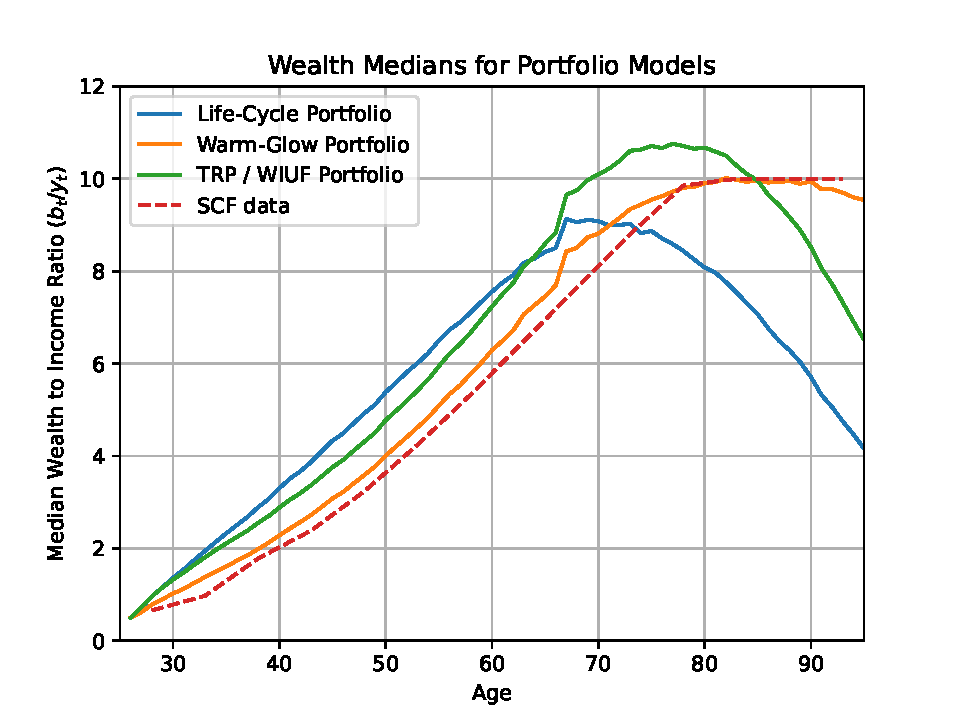
\includegraphics[width=0.7\linewidth]{files/median_wealth-d2524c71e6344dd7c4922a55ce47bf79.pdf}
\caption[]{Median Wealth to Income Ratio for different portfolio models. The red line indicates median wealth-to-income ratios for College educated households in the Survey of Consumer Finances. Wealth is \texttt{networth} and income consists of wages, social security, and retirement income.}
\label{medwealth}
\end{figure}

As discussed above, there are multiple model features that can ameliorate or eliminate the wealth drawdown problem, beginning with a simple bequest motive.
The Warm-Glow Portfolio model (orange lines on figures) estimates a much more realistic CRRA coefficient of $\CRRA = 4.65$.
With a strong bequest motive, the Warm-Glow model is able to match the high levels of wealth observed deep into retirement.
That is, these consumers do not quickly draw down their assets because they take great pleasure in passing their estate on to their heirs.
The bequest motive magnitude $\alpha$ and shifter term $\underline{a}$ cannot be \textit{directly} interpreted in human terms, instead requiring an indirect interpretation used in \cite{DeNardi2010} (see their Appendix D).
Consider the extreme case of a model consumer who is \textit{so old} that they can't possibly survive to the next period-- age 120, in our calibration.
Facing certain imminent death, how much should this person consume versus allocate to their bequest?
The form of the warm-glow bequest motive dictates that the optimal mapping from cash-on-hand to consumption is piecewise linear with a single kink: below a certain threshold wealth-to-income ratio, they should \textit{consume all resources}, and then allocate to their bequest a \textit{constant fraction} of any wealth above the threshold.
The estimated $\alpha$ and $\underline{a}$ can be mathematically transformed to find a ``bequest threshold'' of about 0.43 and a ``marginal propensity to bequeath'' of 0.875; that is, a terminally old agent will allocate to their bequest 87.5\% of any wealth above 43\% of their permanent income.
This strong bequest motive at the very end of life propagates backward to more reasonable ages (albeit not as readily quantifiable), and ultimately it applies for essentially \textit{everyone}.
In contrast, the literature has generally found (e.g. \cite{deNardiBequest}) that the bequest motive comes into play only for relatively wealthy households, and is mostly inoperative around median wealth.
This discrepancy might arise because of the simplified approach we have used here, matching \textit{only} the median wealth-to-income ratio by age, rather than wealth levels conditional on income.

Digging deeper, the Warm-Glow model predicts that saving behavior \textit{when young} is strongly motivated by the bequest motive.
Recall from the discussion of the \cite{2023} and \cite{jaherGilded} that very few older people ascribe their wealth-holding behavior to a bequest motive, and yet the Warm-Glow model has the saving choices of \textit{40 year olds} driven by the urge to bequeath.
Even if a model can \textit{mechanically} reproduce observed data features or hit empirical targets, that does not make it ``right'' or ``true,'' especially if its underlying logic is implausible and contradictory to qualitative evidence.
And as discussed above, the bequest motive is inconsistent with an investment advisor's fiduciary duty \textit{to the client}.
We include the Warm-Glow model in our presentation not to advocate for it, but merely to demonstrate that there are \textit{multiple ways} for life-cycle models to generate more realistic wealth trajectories in retirement.

\begin{figure}[!htbp]
\centering
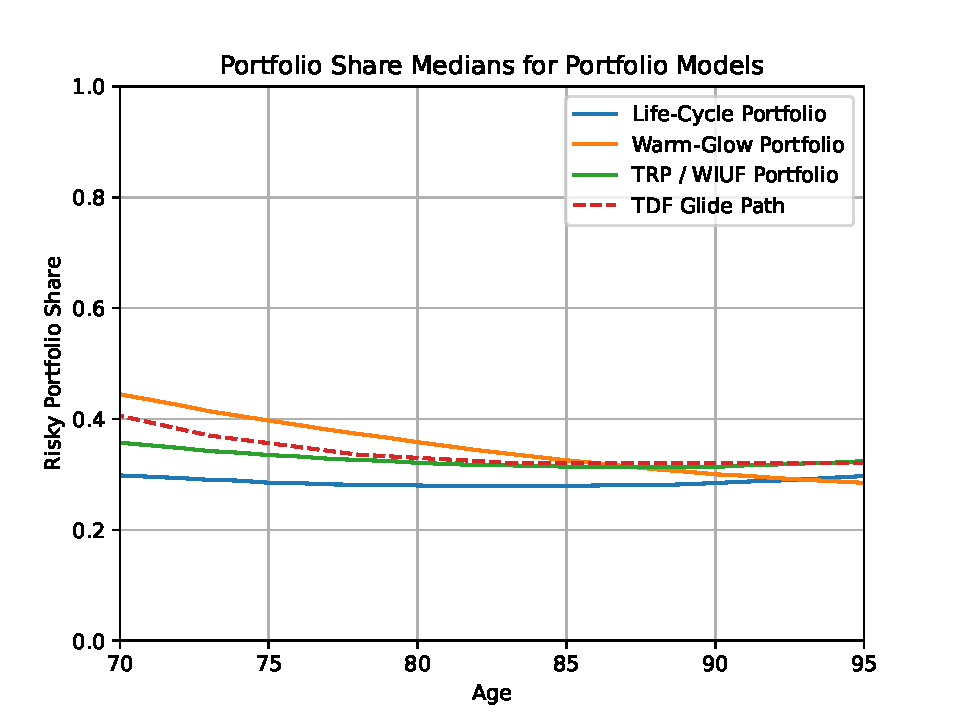
\includegraphics[width=0.7\linewidth]{files/median_share-375a692fb3207501be3ba379fe1a09eb.pdf}
\caption[]{Median Portfolio Share for different portfolio models. The red line shows the target moments from \cite{Aboagye2024}.}
\label{medshare}
\end{figure}

Our preferred specification also has the agents value wealth itself as a motivation to retain assets later in life, but in a way that is more consistent with qualitative responses.
The Wealth-in-Utility-Function (WIUF) / TRP Portfolio model estimates a CRRA $\CRRA$ coefficient of about 4.88 and a wealth share of utility $\delta$ coefficient of 0.16.
This result is significant because the CRRA $\CRRA$ coefficient required to match the wealth accumulation patterns is significantly lower than that of the standard Life-Cycle Portfolio choice model, whose high CRRA $\CRRA$ has long been a puzzle in the literature.
As seen in Figure~\ref{medwealth}, the WIUF / TRP model (green line) does not need to overshoot wealth accumulation in early life by nearly as much as the basic LCP model, as agents want to retain assets in retirement to generate utility directly.
Compared to the Warm-Glow model, the WIUF / TRP specification does predict more wealth accumulation early in life, but for more immediate reasons: young consumers value money and liquidity \textit{now}, rather than saving at age 35 to leave a large bequest at age 85.

Moreover, because the CRRA parameter doesn't need to be so high, the WIUF model can better match the target risky assets share moments (red dashed line in Figure~\ref{medshare}), which come from \cite{Aboagye2024}.
That paper presents the typical glidepath of target-date funds (TDFs) which provide a basis for much of commercial financial advice.
While the whole life-cycle glidepath is provided in \cite{Aboagye2024}, here we only target (and plot) those moments starting at age 70.
The model fit with respect to risky asset share is comparable for the Warm-Glow model, generally matching the level and recommended shallow downward slope.
The basic LCP model, however, badly fits the risky asset share too low due to the high $\CRRA$ value needed in its attempt to match the life-cycle wealth pattern.

\section{Conclusion}

To thoughtful academics, it has long been disturbing that the financial advice industry has paid so little attention to our hard work in constructing and solving impressively sophisticated dynamic stochastic optimization models of financial behavior.
Those of us with a bit of humility have always suspected that the failure has been on our side: If all we could offer was models that produced risible advice like ``everyone should spend down their wealth to zero and live pension-check to pension-check,'' while financial analysts' real world experience told them that such advice would get them fired, then it was reasonable to disregard the academic literature.

The thesis of this paper, however, is that a confluence of factors has now finally brought us to a point where state-of-the-art mathematical/computational life-cycle optimization models can provide advice that makes sense-- so long as the model assumptions are also disciplined by survey data and the practical knowledge of financial advisors.

Much more remains to be done to improve the models further; for example, a question of great practical importance that is now just at the edge of possibility of being computationally solved is to calculate the implications of nonfinancial (principally, housing) wealth for optimal financial choice.
Because homeownership is such a complex phenomenon, the academic literature is only now reaching the point at which it may be possible to answer questions like, ``If I own a house, how should I modify my spending and portfolio plans to take that into account?''
We do know the \textit{direction} of the effect.
\cite{kimballStandardRA} shows that the addition of a new uncontrollable risk reduces the optimal choice of exposure to controllable risks like the stock market.
But \textit{by how much} one's stock exposure should be reduced because of house-price risk can only be answered by solving a quantitatively plausible model.

It would be a better world if financial advice could be justified as reflecting the mathematically optimal solution to a well-defined problem.
Not only would academics have the satisfaction of knowing that they had finally come close to fulfilling the vision of Modligliani and Brumberg 70 years ago.
Financial analysts could also sleep more soundly in the knowledge that the advice they were giving were what many people probably think it already is: The adaptation to the client's particular circumstances of the advice that is the best that can be delivered by the latest high-tech computational optimization tools.

The time seems ripe for a much closer collaboration between academia and the financial industry in building this better world.  This paper's open-source code, built with the associated open-source \href{https://econ-ark.org}{Econ-ARK} project's tools, would be a good place to start.\footnote{We are grateful to the Sloan Foundation and to T Rowe Price for generous funding of the toolkit.}



\bibliographystyle{unsrtnat}
\bibliography{main.bib}

\end{document}
